\documentclass{article}
\usepackage{graphicx}
\usepackage{listings,xcolor}
\usepackage{inconsolata}

\definecolor{dkgreen}{rgb}{0,.6,0}
\definecolor{dkblue}{rgb}{0,0,.6}
\definecolor{dkyellow}{cmyk}{0,0,.8,.3}

\lstset{
	language        = php,
	basicstyle      = \small\ttfamily,
	keywordstyle    = \color{dkblue},
	stringstyle     = \color{red},
	identifierstyle = \color{dkgreen},
	commentstyle    = \color{gray},
	emph            =[1]{php},
	emphstyle       =[1]\color{black},
	emph            =[2]{if,and,or,else},
	emphstyle       =[2]\color{dkyellow}}





\begin{document}
	
	\title{Webprojekt Dokumentation}
	\author{Vincent Manz}
	
	\maketitle

	
	\section{Registrierung und Login}
	Die Registrierung eines Users wurde mit PHP umgesetzt, dabei wurde zuerst ein einfache HTML-Formular erstellt um die vom User eingegebenen Registrierungsdaten an den Server zu \"ubertragen, wobei es ebenfalls zur Auswertung des HTML-Formulars durch den Server kommt. 
	Das nachfolgende Listing zeigt das HTML-Formular:
	\begin{lstlisting}[language=PHP]
	<form action="<?=$_SERVER['PHP_SELF']?>" method="post">
	Username: <input type="text" name="username" /><br />
	Password: <input type="password" name="password" /><br />
	First name: <input type="text" name="first_name" /><br />
	Last name: <input type="text" name="last_name" /><br />
	Email: <input type="type" name="email" /><br />
	
	<input type="submit" name="submit" value="Register" />
	</form>
	\end{lstlisting}
	Wie aus dem Code zu entnehmen ist, werden f\"ur die Registrierung Username, Passwort, Vor- und Zuname und die Email-Adresse des Users \"ubertragen. Durch die Definition des Passwort Eingeabefeld mit \textit{type="password"} wird ein maskieren der eingegebenen Zeichen mit Punkten erreicht wie folgende Abbildung zeigt:
	\newline
	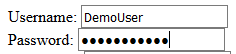
\includegraphics[width=0.5\textwidth]{abb01.png}
	
	Nachdem der User seine Daten zur Registrierung eingegeben hat, werden diese an den Server gesendet. Der Server baut eine Verbindung zur \textit{MySQL}-Datenbank auf, dabei greift er auf eine zuvor erstellte Konfigurationsdatei zu und liest die ben\"otigten Informationen wie z.B. denn Datenbankuser und dessen Passwort aus. Anschlie{\ss}end wird die Verbindung zu Datenbank \"uberpr\"uft. Das nachfolgende Listing zeigt die beschriebene Funktion:
	\begin{lstlisting}
	## Verbindung zur DB aufbauen
	$mysqli = new mysqli(DB_HOST, DB_USER, DB_PASS, DB_NAME);
	# Überprüfe die Verbindung
	if ($mysqli->connect_errno) {
		echo "<p>MySQL error: {$mysqli->connect_errno}"+
		" : {$mysqli->connect_error}</p>";
		exit();
	}
	\end{lstlisting}
	
	Nachdem die Verbindung zur Datenbank \"uberpr\"uft wurde, wird eine Datenbankabfrage vorbereitet, dabei werden die Daten des HTML-Formulars in Variablen gespeichert. Nun wird mittels einer Else-If-Verzweigung \"uberpr\"uft, ob ein Uset mit dem selben Usernamen oder der selben Email-Adresse bereits existiert, damit sich kein User mit denn selben Informationen ein weiteres mal registrieren kann und die Datenkonsistenz gew\"ahrleiset ist. Durch das \textit{echo}-Kommando wird eine entsprechende Information ausgegeben, sollte es bereits existente Eintr\"age geben. Folgendes Listing zeigt den beschrieben Code:
	\newline
	
	\begin{lstlisting}
## Datenbankabfrage:
# Vorbereiten der Daten
$username   = $_POST['username'];
$password   = $_POST['password'];
$first_name = $_POST['first_name'];
$last_name  = $_POST['last_name'];
$email      = $_POST['email'];
	
# Testen ob Username oder Email-Adresse existieren
$exists = 0;
$result = $mysqli->query("SELECT username from users WHERE username = '{$username}'[...]
if ($result->num_rows == 1) {
$exists = 1;
$result = $mysqli->query("SELECT email from users WHERE email = '{$email}' LIMIT 1");
if ($result->num_rows == 1) $exists = 2;    
} else {
$result = $mysqli->query("SELECT email from users WHERE email = '{$email}' LIMIT 1");
if ($result->num_rows == 1) $exists = 3;
}

if ($exists == 1) echo "<p>Username existiert bereits!</p>";
else if ($exists == 2) echo "<p>Username und Email existieren bereits!</p>";
else if ($exists == 3) echo "<p>Email existiert bereits!</p>";
\end{lstlisting}

Nachdem sichergestellt wurde, dass die Daten f\"ur die Erstellung eines neuen Users geeignet sind, wird ein neuer Datenbankeintrag mit den Daten aus dem HTML-Formular erstellt. Anschlie{\ss}end wird eine Meldung ausgegeben, welche dem User mitteilt, das die Registrierung erfolgreich war:
\begin{lstlisting}
# Eintrag in Datenbank erstellen
$sql = "INSERT  INTO `users` (`id`, `username`, `password`, `first_name`, `last_name`, `email`) 
VALUES (NULL, '{$username}', '{$password}', '{$first_name}', '{$last_name}', '{$email}')";

$timestamp = date("F j, Y, g:i a");

setcookie( "cookie[timeOfReg]", $timestamp );

if ($mysqli->query($sql)) {
	echo "<p>Erfolgreich registriert!</p>";
} else {
echo "<p>MySQL error: {$mysqli->errno} : {$mysqli->error}</p>";
exit();
}
\end{lstlisting}
Im Coding wird auch ein Cookie gesetzt, dazu mehr im Abschnitt, welches sich mit dem Setzen und der Auswertung eines Cookies besch\"aftigt.
	

	
\end{document}